
\newpage
\section{Evidence}

\subsection{Primary Requirements}
\begin{figure}[h]
    \centering
    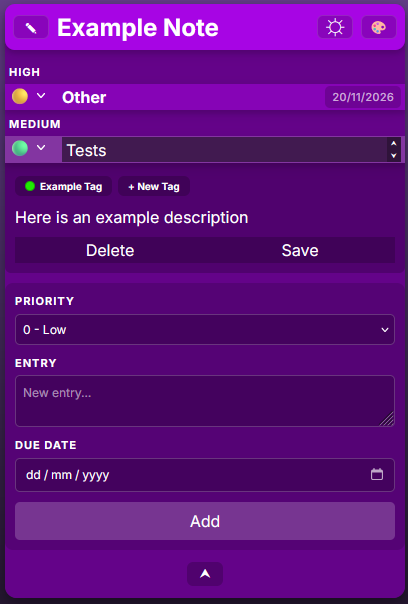
\includegraphics[width=0.65\linewidth]{Images/Evidence/Primary Requirements/Note Example.png}
    \caption{Note Example}
    \label{fig:NoteExample}
\end{figure}


\newpage
\subsubsection{Task Status}

Four tasks were assigned each of the statuses: 'Not Started', 'In Progress', 'Completed', and 'Blocked', demonstrated in \figref{fig:StatusProof}, which confirmed that all states are functional, as well as the selector.

\begin{figure}[h]
    \centering
    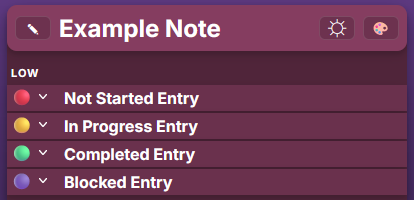
\includegraphics[width=0.35\linewidth]{Images/Evidence/Primary Requirements/Status Proof.png}
    \caption{Status Example}
    \label{fig:StatusProof}
\end{figure}


\subsubsection{Task Priority}

Eight tasks were created with varying priority levels. Another task was created and moved between priorities to verify priority modification was functional. (\figref{fig:PriorityProof})

\begin{figure}[h]
    \centering
    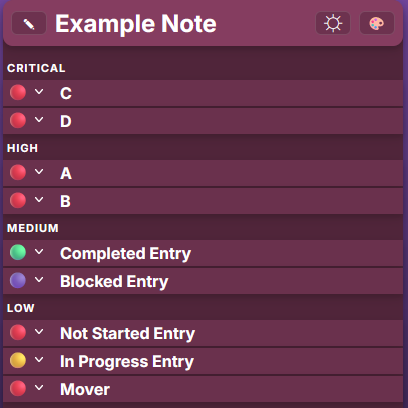
\includegraphics[width=0.35\linewidth]{Images/Evidence/Primary Requirements/Priority Proof.png}
    \caption{Priority Example}
    \label{fig:PriorityProof}
\end{figure}


\subsubsection{Task Descriptions}

Task descriptions can be edited by opening an entry and clicking on the description, as seen in \figref{fig:NoteExample}.

To verify functionality, several entries descriptions were edited, and each was checked to ensure description remained after clicking off the entry, as seen in \figref{fig:DescriptionProof}

\begin{figure}[h]
    \centering
    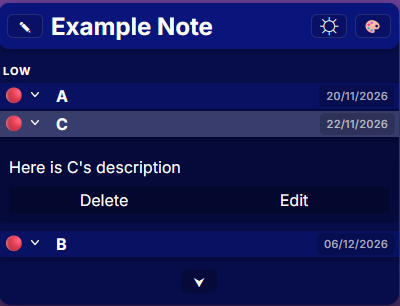
\includegraphics[width=0.35\linewidth]{Images/Evidence/Primary Requirements/DescriptionProof.png}
    \caption{Description Example}
    \label{fig:DescriptionProof}
\end{figure}




\subsection{Organizational Features}
\subsubsection{Task Tags}

Task tags can be added by editing an entry and pressing add tag, or removed by clicking on the tag. The colour can be changed by clicking on the coloured circle. Creating or deleting tags occurs in the add tag menu, with an X to delete, and the '\textit{+ Create new tag}' button on the bottom to create, as seen in \figref{fig:NoteExample}.

To verify functionality, several tags were created and applied to different entries, as seen in \figref{fig:TagProof}.

\begin{figure}[h]
    \centering
    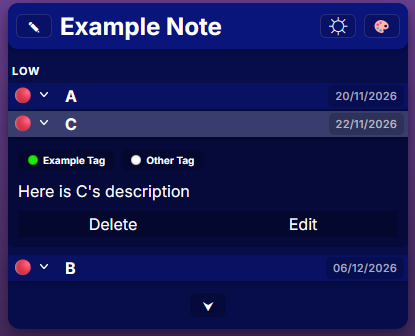
\includegraphics[width=0.4\linewidth]{Images/Evidence/Organizational Features/TagProof.png}
    \caption{Tag Example}
    \label{fig:TagProof}
\end{figure}




\subsubsection{Dashboard}

The dashboard allows users to see how many entries are in the current book, filtered by status, priority, or by tag, as seen in \figref{fig:Dashboard}.

To verify functionality, several entries were changed while the dashboard was open, and counts were checked to be correct.

\begin{figure}[h]
    \centering
    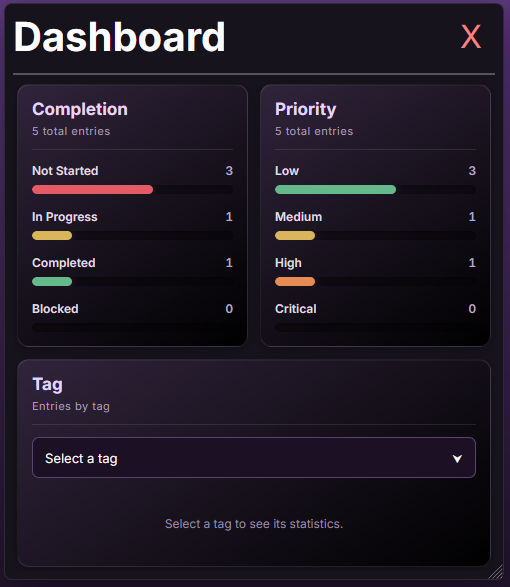
\includegraphics[width=0.5\linewidth]{Images/Evidence/Organizational Features/Dashboard.png}
    \caption{Dashboard Evidence}
    \label{fig:Dashboard}
\end{figure}





\subsection{Authentication and Security}
\subsubsection{User Login}

Users can log in through a simple UI. Functionality was tested with multiple accounts to verify successful authentication and correct loading of books and notes, as seen in \figref{fig:LoginScreen} and \figref{fig:LoginSuccess}. 

Invalid credentials are rejected, requiring user to reattempt. Return messages do not reveal whether an account exists, preventing username enumeration.

\begin{figure}[h]
    \centering
    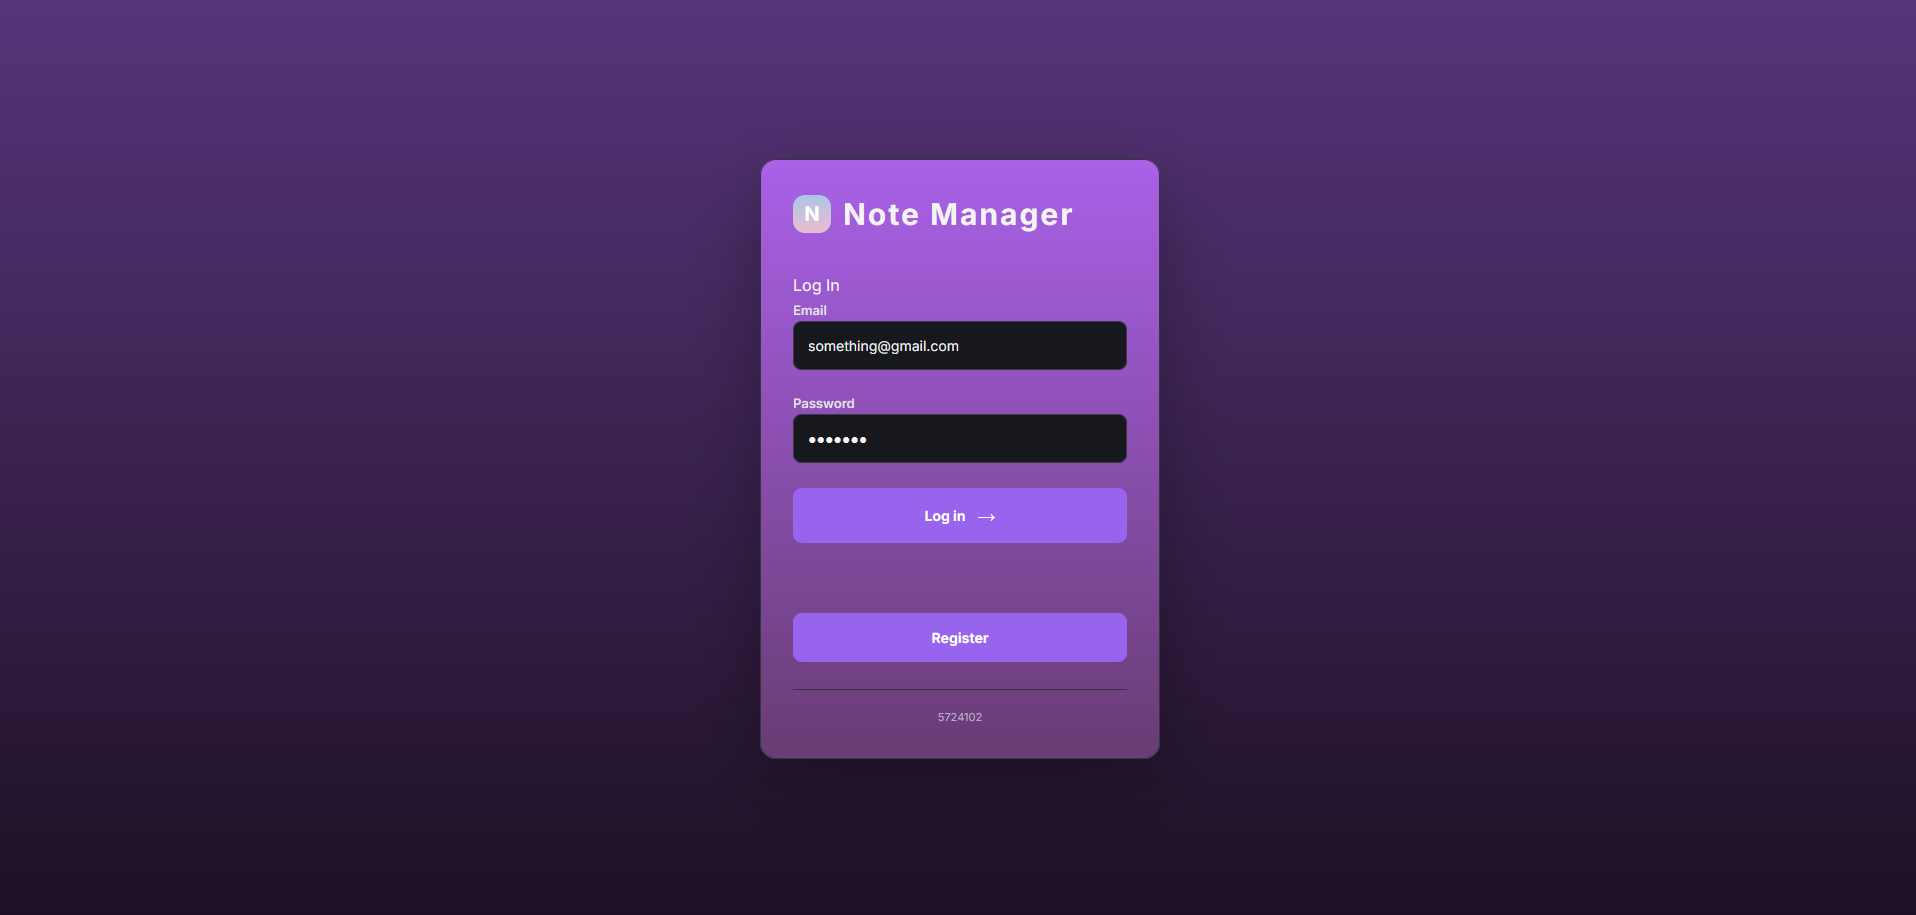
\includegraphics[width=1\linewidth]{Images/Evidence/Authentication and Security/LoginProofA.png}
    \caption{Login Screen}
    \label{fig:LoginScreen}
\end{figure}
\begin{figure}[h]
    \centering
    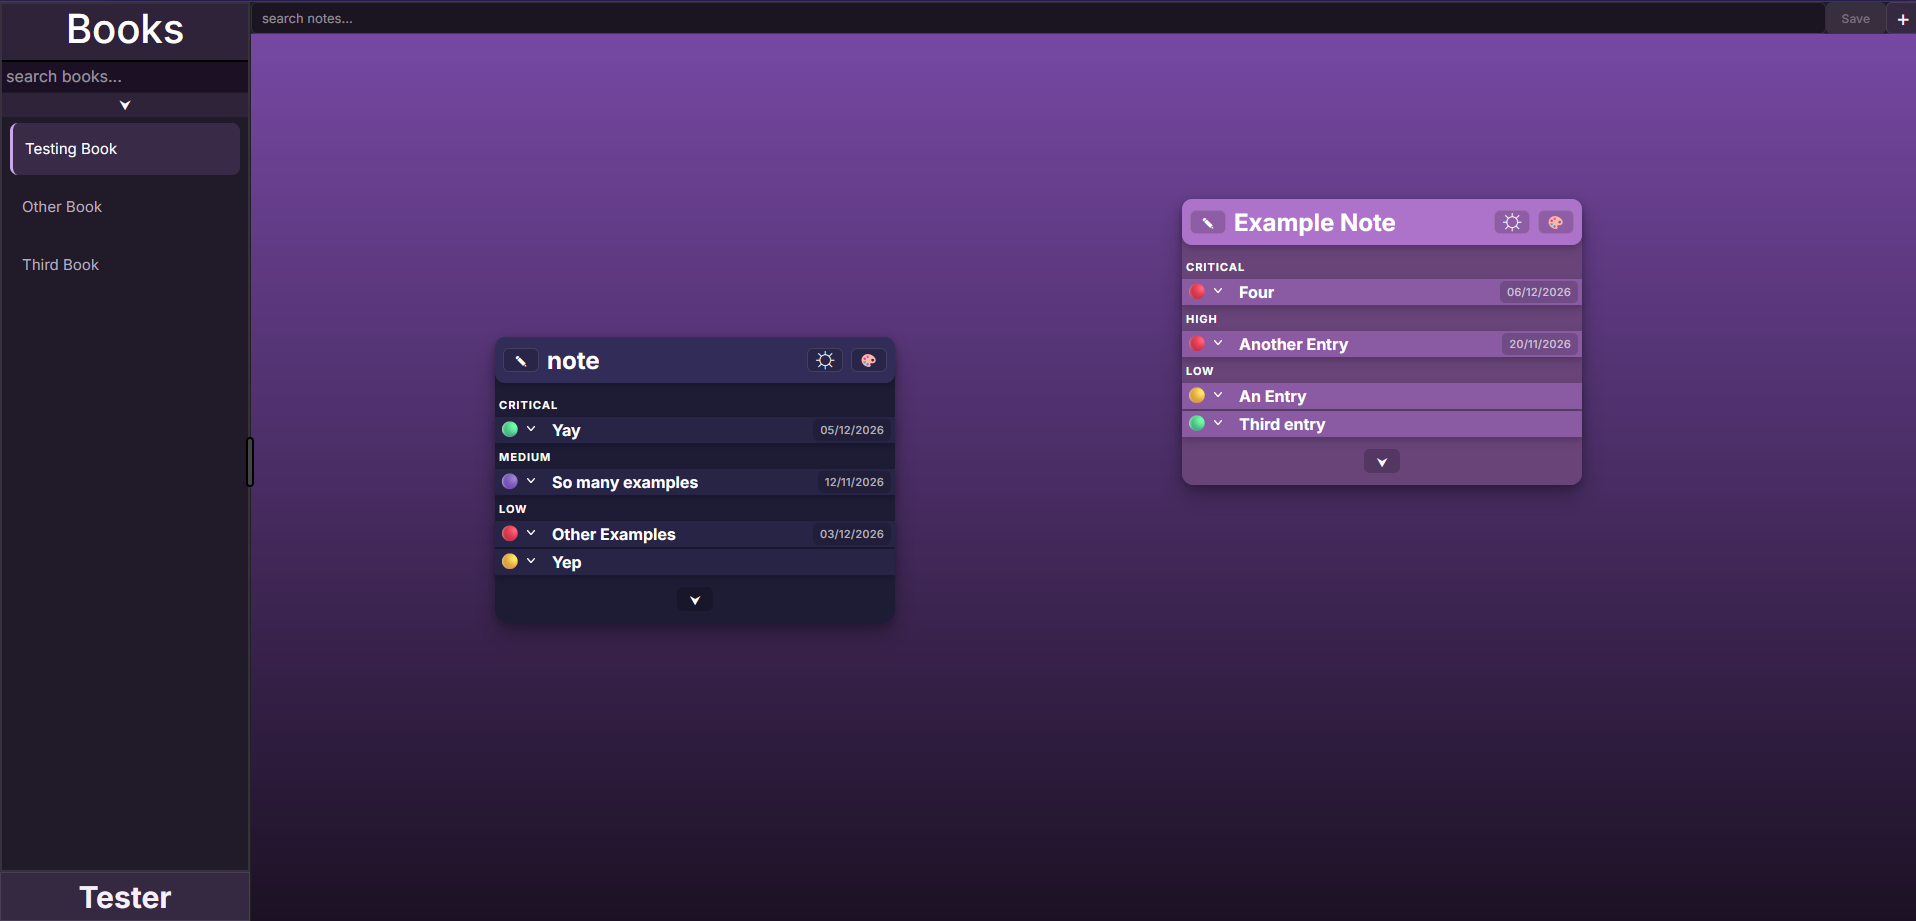
\includegraphics[width=1\linewidth]{Images/Evidence/Authentication and Security/SuccessfulLogin.png}
    \caption{Successful login and loading}
    \label{fig:LoginSuccess}
\end{figure}





\subsubsection{Secure Password Handling}

While not currently enabled, when in production HTTPS will be used to transmit the users plaintext password to the server.

When the password reaches the server, it verifies it against the Argon2 hashed password in the database, if valid then it allows login, else it denies. The plaintext password is never stored, as seen in \figref{fig:LoginAPI} and \figref{fig:LoginDB}.

\begin{figure}[h]
    \centering
    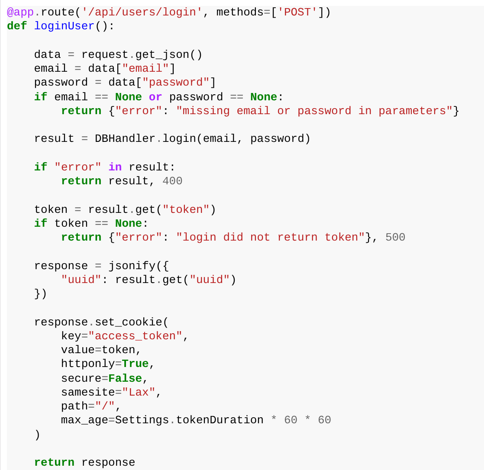
\includegraphics[width=0.7\linewidth]{Images/Evidence/Authentication and Security/LoginAPI.png}
    \caption{Login API}
    \label{fig:LoginAPI}
\end{figure}
\begin{figure}[h]
    \centering
    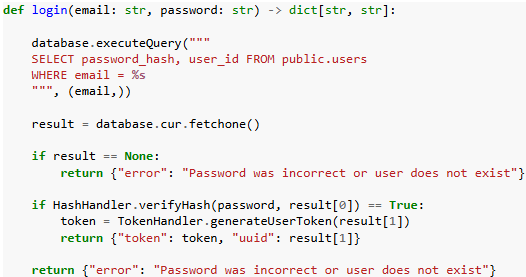
\includegraphics[width=0.7\linewidth]{Images/Evidence/Authentication and Security/LoginDB.png}
    \caption{Login DB}
    \label{fig:LoginDB}
\end{figure}




\subsubsection{Session and Token Management}

Sessions are continued via a HTTP only cookie that contains a JWT that authenticates the user. The user receives this cookie on login, as seen in \figref{fig:LoginAPI}. This JWT is handled by a JWT handler class, improving modularity, as seen in \figref{fig:TokenHandler}.

\begin{figure}[h]
    \centering
    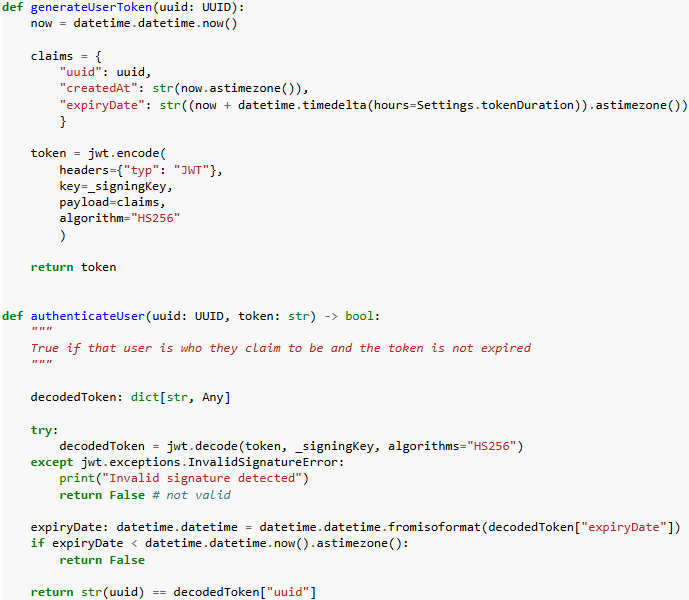
\includegraphics[width=1\linewidth]{Images/Evidence/Authentication and Security/TokenHandler.png}
    \caption{Token Handler Functions}
    \label{fig:TokenHandler}
\end{figure}


\subsubsection{Enumeration Prevention}

API responses could allow for username enumeration if different status codes were returned for existing users and those that don't (401 vs 404).